\chapter{图}
在ACM竞赛中,图一般使用邻接矩阵表示,代码框架如下;

\begin{Codex}[label=graph.c]
#define MAXN 100  // 顶点最大个数

int n; // 顶点个数
int G[MAXN][MAXN]; // 邻接矩阵
int visited_edges[MAXN][MAXN]; // 边的访问历史记录
int visited_vertices[MAXN]; // 顶点的访问历史记录
\end{Codex}

\section{深度优先搜索} %%%%%%%%%%%%%%%%%%%%%%%%%%%%%%
图的深度优先搜索的代码框架如下:

\begin{Codex}[label=graph.c]
/**
 * @brief 图的深度优先搜索代码框架,搜索边.
 * @param[in] u 出发顶点
 * @param[in] n 顶点个数
 * @param[in] G 图的临街举着
 * @param[in] visited 边的访问历史记录
 * @return 无
 * @remark 在使用的时候,为了降低递归的内存占用量,可以把
 * n, G, visited 抽出来作为全局变量
 */
void dfs(const int u, 
                const int n, const int G[][MAXN], int visited[][MAXN]) {
    int v;
    for(v = 0;  v < n; v++) if(G[u][v] && !visited[u][v]) {
        visited[u][v] = visited[v][u] = 1; // 无向图用这句
        // visited_edges[u][v] = 1; // 有向图用这句
        dfs(v, n, G, visited);
        // 这里写逻辑代码
        // printf("%d %d\n", u, v);
    }
}

/**
 * @brief 图的深度优先搜索代码框架,搜索顶点.
 * @param[in] u 出发顶点
 * @param[in] n 顶点个数
 * @param[in] G 图的临街举着
 * @param[in] visited 顶点的访问历史记录
 * @return 无
 * @remark 在使用的时候,为了降低递归的内存占用量,可以把
 * n, G, visited 抽出来作为全局变量
 */
void dfs(const int u, 
                const int n, const int G[][MAXN], int visited[MAXN]) {  
    int v;
    visited[u] = 1;
    for(v = 0;  v < n; v++) if(G[u][v] && !visited[v]) {
        dfs(v, n, G, visited);
        // 这里写逻辑代码
        // printf("%d %d\n", u, v);
    }
}
\end{Codex}

\subsection{黑白图像}

\subsubsection{描述}
输入一个n*n的黑白图像(1表示黑丝,0表示白色),任务是统计其中八连块的个数。
如果两个黑格子有公共边或者公共定点,就说它们属于同一个八连块。如图~\ref{fig:blackwhiteImage}所示的
黑白图像中有3个八连块。

\begin{center}
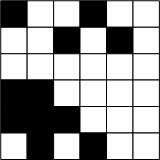
\includegraphics[width=90pt]{blackwhite-image.jpg}\\
\figcaption{拥有3个八连块的黑白图}\label{fig:blackwhiteImage}
\end{center}

\subsubsection{代码}
\begin{Codex}[label=blackwhite_image.c]
#include <stdio.h>
#include <string.h>

#define MAXN 16

int n;
// 黑白图,1 表示黑色,0表示白色,加一圈0,用于判断出界
int G[MAXN + 1][MAXN + 1];
// 记录格子(x,y)是否已经被访问过
int visitied[MAXN][MAXN];

void dfs(const int x, const int y) {
    // 曾经访问过这个格子,或者当前格子是白色
    if(G[x][y] == 0 || visitied[x][y] == 1)  return;
    
    visitied[x][y] = 1; // 标记(x,y)已访问过
    // 递归访问周围的8个格子
    dfs(x - 1, y - 1); // 左上角
    dfs(x - 1, y); // 正上方
    dfs(x - 1, y + 1); // 右上角
    dfs(x, y - 1); // 左边
    dfs(x, y + 1); // 右边
    dfs(x + 1, y - 1); // 左下角
    dfs(x + 1, y); // 正下方
    dfs(x + 1, y + 1); // 右下角
}

/*
Sample Input
6
100100
001010
000000
110000
111000
010100
Sample Output
3
*/
int main() {
    int i, j;
    char s[MAXN]; // 矩阵的一行
    int count = 0; // 八连块的个数

    scanf("%d", &n);
    memset(G, 0, sizeof(G));
    memset(visitied, 0, sizeof(visitied));

    for(i = 0; i < n; ++i) {
        scanf("%s", s);
        for(j = 0; j < n; ++j) {
            G[i + 1][j + 1] = s[j] - '0'; // 把图像往中间挪一点,空出一圈白格子
        }
    }


    for(i = 1; i <= n; ++i) {
        for(j = 1; j <= n; ++j) {
            if(visitied[i][j] == 0 && G[i][j] == 1) {
                count++;
                dfs(i, j);
            }
        }
    }
    printf("%d\n", count);
    return 0;
}
\end{Codex}

\subsubsection{相关的题目}
与本题相同的题目:
\begindot
\item 《算法竞赛入门经典》\footnote{刘汝佳,算法竞赛入门经典,清华大学出版社,2009} 第107页6.4.1节
\item  TODO
\myenddot

与本题相似的题目:
\begindot
\item  TODO
\myenddot

\subsection{欧拉回路}

\subsubsection{描述}
本题是 UVA 10054 - The Necklace。

My little sister had a beautiful necklace made of colorful beads. Two successive beads in the 
necklace shared a common color at their meeting point. The figure below shows a segment of 
the necklace:

\centerline{\fbox{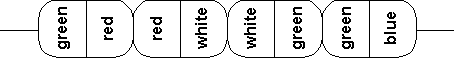
\includegraphics[width=240pt]{uva10054.png}}}

But, alas! One day, the necklace was torn and the beads were all scattered over the floor. 
My sister did her best to recollect all the beads from the floor, but she is not sure 
whether she was able to collect all of them. Now, she has come to me for help. She wants
 to know whether it is possible to make a necklace using all the beads she has in the same
 way her original necklace was made and if so in which order the bids must be put.

Please help me write a program to solve the problem.

\subsubsection{Input}
The input contains T test cases. The first line of the input contains the integer T.

The first line of each test case contains an integer $N(5 \leq N \leq 1000)$ giving the number of beads 
my sister was able to collect. Each of the next N lines contains two integers describing 
the colors of a bead. Colors are represented by integers ranging from 1 to 50.

\subsubsection{Output}
For each test case in the input first output the test case number as shown in the sample output. Then 
if you apprehend that some beads may be lost just print the sentence ``some beads may be lost" on a 
line by itself. Otherwise, print N lines with a single bead description on each line. Each bead 
description consists of two integers giving the colors of its two ends. For $1 \leq i \leq N_1$, the second integer 
on line i must be the same as the first integer on line i + 1. Additionally, the second integer 
on line N must be equal to the first integer on line 1. Since there are many solutions, any one
 of them is acceptable.

Print a blank line between two successive test cases.

\subsubsection{Sample Input}
\begin{Code}
2
5
1 2
2 3
3 4
4 5
5 6
5
2 1
2 2
3 4
3 1
2 4
\end{Code}

\subsubsection{Sample Output}
\begin{Code}
Case #1
some beads may be lost

Case #2
2 1
1 3
3 4
4 2
2 2
\end{Code}

\subsubsection{分析}
这题就是欧拉回路+打印路径。

如果能从图的某一顶点出发,每条边恰好经过一次,这样的路线称为\textbf{欧拉道路}(Eulerian Path)。
如果每条边恰好经过一次,且能回到起点,这样的路线称为\textbf{欧拉回路}(Eulerian Circuit)。

对于无向图G,当且仅当G是连通的,且最多有两个奇点,则存在欧拉道路。
如果有两个奇点,则必须从其中一个奇点出发,到另一个奇点终止。

如果没有奇点,则一定存在一条欧拉回路。

对于有向图G,当且仅当G是连通的,且每个点的入度等于出度,则存在欧拉回路。

如果有两个顶点的入度与出度不相等,且一个顶点的入度比出度小1,另一个顶点的入度比出度大1,此时,
存在一条欧拉道路,以前一个顶点为起点,以后一个顶点为终点

\subsubsection{代码}
\begin{Codex}[label=eulerian_circuit.c]
#include <stdio.h>
#include<string.h>

#define MAXN 51  // 顶点最大个数

int G[MAXN][MAXN];
int visited_vertices[MAXN]; 
int visited_edges[MAXN][MAXN];
int count[MAXN]; // 顶点的度

void dfs(const int u) {  
    int v;
    visited_vertices[u] = 1;
    for(v = 0;  v < MAXN; v++) if(G[u][v] && !visited_vertices[v]) {
        dfs(v);
    }
}

/*
 * @brief 欧拉回路,允许自环和重复边
 * @param[in] u 起点
 * @return 无
 */
void euler(const int u){
    int v;
    for(v = 0; v < MAXN; ++v) if(G[u][v]){
        --G[u][v]; --G[v][u]; // 这个技巧,即有visited的功能,又允许重复边
        euler(v);
        // 逆向打印,或者存到栈里再打印
        printf("%d %d\n", u, v);
    }
}

int main() {
    int T, N, a, b;
    int i;
    int cases=1;
    scanf("%d",&T);
    while(T--) {
        int flag = 1; // 结点的度是否为偶数
        int flag2 = 1; // 图是否是连通的
        
        memset(G, 0, sizeof(G));
        memset(count, 0, sizeof(count));

        scanf("%d",&N);
        for(i = 0; i < N; ++i){
            scanf("%d %d", &a, &b); 
            ++G[a][b];
            ++G[b][a];
            ++count[a];
            ++count[b];
        }

        printf("Case #%d\n", cases++);

        // 欧拉回路形成的条件之一,判断结点的度是否为偶数
        for(i=0; i<MAXN; ++i) {
            if(count[i] & 1){
                flag = 0;
                break;
            }
        }
        // 检查图是否连通
        if(flag) {
            memset(visited_vertices, 0, sizeof(visited_vertices));
            memset(visited_edges, 0, sizeof(visited_edges));

            for(i=0; i< MAXN; ++i) 
                if(count[i]) { 
                    dfs(i);
                    break; 
                }
            for(i=0; i< MAXN; ++i){
                if(count[i] && !visited_vertices[i]) {
                    flag2 = 0; 
                    break;
                }
            }
        }
        if (flag && flag2) {
            for(i = 0; i < MAXN; ++i) if(count[i]){
                euler(i);
                break;
            }
        } else {
            printf("some beads may be lost\n");
        }

        if(T > 0) printf("\n");
    }
    return 0;
}
\end{Codex}

\subsubsection{相关的题目}
与本题相同的题目:
\begindot
\item 《算法竞赛入门经典》\footnote{刘汝佳,算法竞赛入门经典,清华大学出版社,2009} 第111页6.4.4节
\item  TODO
\myenddot

与本题相似的题目:
\begindot
\item  UVa 10129 Play on Words, \myurl{http://t.cn/zTInBDX}
\myenddot


\section{广度优先搜索} %%%%%%%%%%%%%%%%%%%%%%%%%%%%%%



\section{最小生成树} %%%%%%%%%%%%%%%%%%%%%%%%%%%%%%
“最小”指的是边的权值之和最小。

构造最小生成树(Minimum Spanning Tree, MST)有多种算法。其中多数算法利用了最小生成树的一个性质(简称为MST性质):假设$N=(V, E)$是一个连通网,$U$是顶点集$V$的一个非空子集。若$(u, v)$是一条具有最小权值的边,其中$u \in U, v \in V-U$,则必存在一颗包含边$(u, v)$的最小生成树。

Prim算法和Kruskal算法是两个利用MST性质构造最小生成树的算法。它们都属于贪心法。

\subsection{Prim算法}
假设$N=(V, E)$是一个连通网,$TE$是$N$上最小生成树中边的集合。算法从$U={u_0}(u_0 \in V), TE=\{\}$开始,重复执行下述操作:在所有$u \in U, v \in V-U$的边$(u, v) \in E$中找一条代价最小的边$(u_0, v_0)$并入集合$TE$,同时$v_0$并入U,直至$U=V$为止。此时$TE$中必有$n-1$条边,则$T=(V, TE)$为$N$的最小生成树。
为实现这个算法需附设一个数组\fn{closedge},以记录从$U$到$V-U$具有最小代价的边。对每个顶点$v_i \in V-U$,在辅助数组中存在一个相应分量\fn{closedge[i-1]},它包括两个域,其中\fn{lowcost}存储该边上的权。显然,$closedge[i].lowcost=\min\left\{cost(u, v_i), u \in U\right\}$。\fn{adjvex}域存储该边依附的在U中的顶点。

图 \ref{fig:prim}所示为按Prim算法构造网的一棵最小生成树的过程,在构造过程中辅助数组中各分量值的变化如表\ref{tab:prim}所示。

\begin{center}
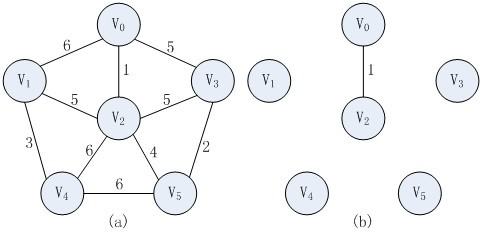
\includegraphics[width=240pt]{prim1.png}\\
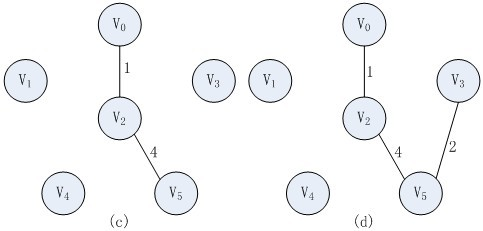
\includegraphics[width=240pt]{prim2.png}\\
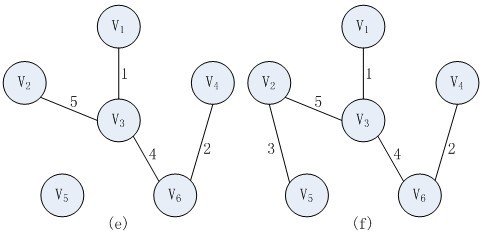
\includegraphics[width=240pt]{prim3.png}\\
\figcaption{Prim算法构造最小生成树的过程}\label{fig:prim}
\end{center}

\begin{center}
\tabcaption{构造最小生成树过程中辅助数组的变化}
\label{tab:prim}
\begin{tabular}{|c|cccccccc|}
\hline
\textbf{\diagbox{closedge}{i}} & \textbf{1} & \textbf{2} & \textbf{3} & \textbf{4}& \textbf{5}& \textbf{U}& \textbf{U-V}& \textbf{k}\\
\hline
adjvex & $v_0$ & $v_0$ & $v_0$ & & & $v_0$ & $\{v_1,v_2,v_3,v_4,v_5\}$ & \multirow{2}{*}{2} \\
lowcost & 6 & 1 & 5 & & & & & \\
\hline
adjvex & $v_2$ & & $v_1$ & $v_2$ & $v_2$ & $\{v_0,v_2\}$ & $\{v_1,v_3,v_4,v_5\}$ & \multirow{2}{*}{5} \\
lowcost & 5 & 0 & 5 & 6 & 4 & & & \\
\hline
adjvex & $v_2$ & & $v_6$ & $v_2$ & & $\{v_0,v_2,v_5\}$ & $\{v_1,v_3,v_4\}$ & \multirow{2}{*}{3} \\
lowcost & 5 & 0 & 2 & 6 & 0 & & & \\
\hline
adjvex & $v_2$ & & & $v_2$ & & $\{v_0,v_2,v_5,v_3\}$ & $\{v_1,v_4\}$ & \multirow{2}{*}{1} \\
lowcost & 5 & 0 & 0 & 6 & 0 & & & \\
\hline
adjvex & & & & $v_1$ & & $\{v_0,v_2,v_5,v_3,v_1\}$ & $\{v_4\}$ & \multirow{2}{*}{4} \\
lowcost & 0 & 0 & 0 & 3 & 0 & & & \\
\hline
adjvex & & & & & & $\{v_0,v_2,v_5,v_3,v_1,v_4\}$ & $\{\}$ & \multirow{2}{*}{} \\
lowcost & 0 & 0 & 0 & 0 & 0 & & & \\
\hline
\end{tabular}
\end{center}


\subsubsection{代码}

\begin{Codex}[label=mgraph_prim1.c]
#include <stdio.h>
#include <stdlib.h>  /* for malloc() */
#include <limits.h>  /* for INT_MAX */

/** 顶点数的最大值*/
#define MAX_VERTICES_NUM 100
/** 边的权值,对无权图,用0或1表示是否相邻;对有权图,则为权值. */
typedef int graph_weight_t;
/** 顶点信息,例如顶点名字. */
typedef char graph_vertex_t;

/**
 *@struct
 *@brief 邻接矩阵.
 */
typedef struct mgraph_t {
    int vertices_num; /* 顶点数*/
    int edges_num; /* 边数*/
    /* 顶点表,存放顶点的信息,如名字等*/
    graph_vertex_t vertices[MAX_VERTICES_NUM];
    /* 邻接矩阵,存放边的信息,如权重等*/
    graph_weight_t matrix[MAX_VERTICES_NUM][MAX_VERTICES_NUM];
    int directed; /* 图(网)的种类,1表示有向,0表示无向*/
} mgraph_t;

mgraph_t g;

typedef struct closedge_t {
    int adjvex; /* 弧头,属于U */
    graph_weight_t lowcost; /* 边 adjvex->本下标 的权值,INT_MIN表示已经加入U */
} closedge_t;

/*
 * @brief 在V-E集合中寻找最小的边
 * @param[in] closedge MST中的边,起点为adjvex,终点为本下标
 * @param[in] n closedge数组的长度
 * @return 找到了则返回弧尾的下标,V-U为空集则返回-1,表示终止
 */
static int min_element(const closedge_t closedge[], int n) {
    int i;
    int min_value = INT_MAX;
    int min_loc = -1;
    for (i = 0; i < n; i++)
        if (closedge[i].lowcost > INT_MIN) {
            if (min_value > closedge[i].lowcost) {
                min_value = closedge[i].lowcost;
                min_loc = i;
            }
        }
    return min_loc;
}

/**
 * @brief Prim算法,求图的最小生成树.
 * @param[in] g 图对象的指针
 * @return MST的边的权值之和
 */
graph_weight_t mgraph_prim(const mgraph_t *g) {
    graph_weight_t sum = 0; /* 权值之和 */
    int i, j;
    int u = 0; /* 从0号顶点出发 */
    const int n = g->vertices_num;
    /* closedge[n],记录从顶点集U到V-U的边*/
    closedge_t* const closedge = (closedge_t*) malloc(n * sizeof(closedge_t));

    /* 辅助数组初始化*/
    for (i = 0; i < n; i++) if (i != u) {
        closedge[i].adjvex = u;
        closedge[i].lowcost = g->matrix[u][i];
    }
    closedge[u].lowcost = INT_MIN; /* 初始, U={u} */

    for (i = 0; i < n; i++) if (i != u) { /* 其余的n-1个顶点*/
        /* 求出TE的下一个顶点k */
        const int k = min_element(closedge, n);
        /* 输出此边 closedge[k].adjvex --> k */
        printf("%c - %c\n", g->vertices[closedge[k].adjvex], g->vertices[k]);
        sum += g->matrix[closedge[k].adjvex][k];
        // sum += closedge[k].lowcost;  // 等价
        closedge[k].lowcost = INT_MIN;  /* 顶点k并入U,表示此边加入TE */
        /* 更新k的邻接点的值,不相邻为无穷大*/
        for (j = 0; j < n; j++) {
            const graph_weight_t w = g->matrix[k][j];
            if (w < closedge[j].lowcost) {
                closedge[j].adjvex = k;
                closedge[j].lowcost = w;
            }
        }
    }
    free(closedge);
    return sum;
}

/* test

输入数据:

7 11
A B 7
A D 5
B C 8
B D 9
B E 7
C E 5
D E 15
D F 6
E F 8
E G 9
F G 11

输出:

A - D : 5
D - F : 6
A - B : 7
B - E : 7
E - C : 5
E - G : 9
Total:39
*/
int main() {
    int i, j, k, m, n;
    char chx, chy;
    int cost;

    /* 读取节点和边的数目 */
    scanf("%d%d", &m, &n);
    getchar(); // 消耗回车键
    g.vertices_num = m;
    g.edges_num = n;
    for (i = 0; i < m; i++) g.vertices[i] = 'A' + i;

    /* 初始化图,所有节点间距离为无穷大 */
    for (i = 0; i < m; i++) {
        for (j = 0; j < m; j++) {
            g.matrix[i][j] = INT_MAX;
        }
    }

    /* 读取边信息 */
    for (k = 0; k < n; k++) {
        scanf("%c %c %d", &chx, &chy, &cost);
        getchar();
        i = chx - 'A';
        j = chy - 'A';
        g.matrix[i][j] = cost;
        g.matrix[j][i] = cost;
    }

    /* 求解最小生成树 */
    printf("Total:%d\n", mgraph_prim(&g));
    return 0;
}
\end{Codex}

\subsubsection{算法分析}
假设网中有$n$个顶点,则第一个进行初始化的循环语句的频度为$n$,第二个循环语句的频度为$n-1$。其中有两个内循环:其一是在\fn{closedge[v].lowcost}中求最小值,其频度为$n-1$;其二是重新选择具有最小代价的边,其频度为$n$。因此Prim算法的时间复杂度为$O(n^2)$,与网中边数无关,因此适用于求边稠密的图的最小生成树。

Prim算法的另一种实现是使用小根堆,其流程是:小根堆中存储一个端点在生成树中,另一个端点不在生成树的边,每次从小根堆的堆顶可选出权值最小的边$(u, v)$,将其从堆中推出,加入生成树中。然后将新出现的所有一个端点在生成树中,一个端点不在生成树的边都插入小根堆中。下一轮迭代中,下一条满足要求的边又上升到堆顶。如此重复$n-1$次,最后建立起该图的最小生成树。该算法的C代码实现如下。

\subsubsection{代码}

\begin{Codex}[label=mgraph_prim2.c]
#include <stdio.h>
#include <stdlib.h>  /* for malloc() */
#include <limits.h>  /* for INT_MAX */

/** 顶点数的最大值*/
#define MAX_VERTICES_NUM 100
/** 边的权值,对无权图,用0或1表示是否相邻;对有权图,则为权值. */
typedef int graph_weight_t;
/** 顶点信息,例如顶点名字. */
typedef char graph_vertex_t;

/**
 *@struct
 *@brief 邻接矩阵.
 */
typedef struct mgraph_t {
    int vertices_num; /* 顶点数*/
    int edges_num; /* 边数*/
    /* 顶点表,存放顶点的信息,如名字等*/
    graph_vertex_t vertices[MAX_VERTICES_NUM];
    /* 邻接矩阵,存放边的信息,如权重等*/
    graph_weight_t matrix[MAX_VERTICES_NUM][MAX_VERTICES_NUM];
    int directed; /* 图(网)的种类,1表示有向,0表示无向*/
} mgraph_t;

mgraph_t g;


/**
 * @struct 边
 */
typedef struct edge_t{
    int tail;  /** 弧尾, from */
    int head;  /** 弧头, to */
    graph_weight_t cost;  /** 权值 */
}edge_t;

static int edge_cmp(const edge_t *e1, const edge_t *e2) {
    const edge_t* const e11 = (const edge_t *)e1;
    const edge_t* const e22 = (const edge_t *)e2;
    return e11->cost - e22->cost;
}

typedef edge_t heap_elem_t; // 元素的类型

/* 等价于复制粘贴,这里为了节约篇幅,使用include,在OJ上提交时请用复制粘贴 */
#include "heap.c"


/**
  * @brief Prim算法,求图的最小生成树.
  * @param[in] g 图对象的指针
  * @return MST的边的权值之和
  */
int mgraph_prim(const mgraph_t *g){
    graph_weight_t sum = 0; /* 权值之和 */
    int u = 0; /* 从0号顶点出发 */
    int i, count = 1;
    edge_t ed;
    heap_t h;
    const int n = g->vertices_num;
    /* 判断顶点是否已经加入最小生成树*/
    int* U = (int *)malloc(n * sizeof(int));
    for(i = 0; i < n; i++) U[i] = 0;
    heap_init(&h, g->edges_num, edge_cmp);

    /* 开始顶点加入U(所以count初始为1) */
    U[u] = 1;
    while (count < n) {
        int v;
        for(v = 0; v < n; v++) if(!U[v]) { /* 若v不在生成树,(u,v)加入堆*/
            ed.tail = u;
            ed.head = v;
            /* tail在树内,head不在树内*/
            ed.cost = g->matrix[u][v];
            heap_push(&h, ed);
        }
        while(!heap_empty(&h) && count < n) {
            /* 从堆中退出最小权值边,存入ed */
            ed = heap_top(&h); heap_pop(&h);
            if(!U[ed.head]) {
                /* 输出生成树TE的边,即此边加入TE */
                printf("%c - %c\n", g->vertices[ed.tail],
                        g->vertices[ed.head]);
                sum += g->matrix[ed.tail][ed.head];
                u = ed.head;
                /* u并入到生成树的顶点集合U */
                U[u] = 1;
                count++;
                break;
            }
        }
    }

    free(U);
    heap_uninit(&h);
    return sum;
}


// test,输入数据和main()函数与 mgraph_prim1.c 相同
// int main() {
// ...
\end{Codex}

\subsubsection{算法分析}
该算法迭代次数为$O(n)$,每次迭代将平均$e/n$条边插入最小堆中,$e$条边从堆中删除,堆的插入和删除操作时间复杂度均为$O(\log_2 e)$,则总的时间复杂度为 $O(e\log_2e)$。

\subsection{Kruskal算法}
假设连通网$N={V, E}$,则令最小生成树的初始状态为只有$n$个顶点而无边的非连通图$T=(V, {})$,图中每个顶点自成一个连通分量。在$E$中选择代价最小的边,若该边依附的顶点落在$T$中不同的连通分量上,则将此边加入到$T$中,否则舍去此边而选择下一条代价最小的边。依次类推,直至T中所有顶点都在同一连通分量上为止。

图\ref{fig:kruskal}所示为Kruskal算法构造一棵最小生成树的过程。

\begin{center}
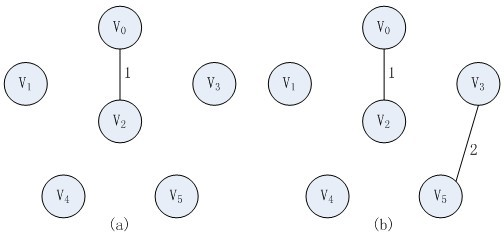
\includegraphics[width=240pt]{kruskal1.png}\\
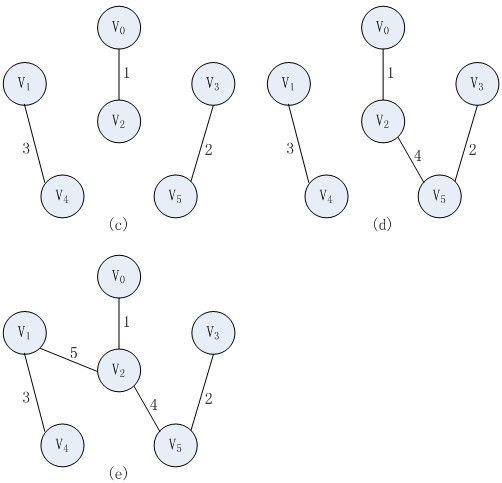
\includegraphics[width=240pt]{kruskal2.png}\\
\figcaption{Kruskal算法构造最小生成树的过程}\label{fig:kruskal}
\end{center}

下面是Kruskal算法的C语言实现。

\subsubsection{代码}

\begin{Codex}[label=mgraph_kruskal.c]
#include <stdio.h>
#include <stdlib.h>  /* for malloc() */
#include <limits.h>  /* for INT_MAX */

/************ 并查集 ************/
/**
  * @brief 初始化并查集.
  * @param[in] s 双亲表示法的数组
  * @param[in] n 数组s的元素个数
  * @return 无
  */
void ufs_init(int s[], int n) {
    int i;
    for(i = 0; i < n; i++) s[i] = -1;
}

/**
  * @brief Find操作,查找包含元素x的树的根.
  * @param[in] s 双亲表示法的数组
  * @param[in] x 要查找的元素
  * @return 包含元素x的树的根
  */
int ufs_find(const int s[], int x) {
    while(s[x] >= 0) {
        x = s[x];
    }
    return x;
}

 /*
  * @brief Union操作,求两个不相交集合的并集.
  * @param[in] s 双亲表示法的数组
  * @param[in] root1 一棵树的根
  * @param[in] root2 另一棵树的根
  * @return 无
  */
void ufs_union(int s[], int root1, int root2) {
    s[root1] += s[root2];
    s[root2] = root1;
}
/************ 并查集 ************/


/** 顶点数的最大值*/
#define MAX_VERTICES_NUM 100
/** 边的权值,对无权图,用0或1表示是否相邻;对有权图,则为权值. */
typedef int graph_weight_t;
#define INFINITY INT_MAX  /* 边权值无穷大 */
/** 顶点信息,例如顶点名字. */
typedef char graph_vertex_t;

/**
 *@struct
 *@brief 邻接矩阵.
 */
typedef struct mgraph_t {
    int vertices_num; /* 顶点数*/
    int edges_num; /* 边数*/
    /* 顶点表,存放顶点的信息,如名字等*/
    graph_vertex_t vertices[MAX_VERTICES_NUM];
    /* 邻接矩阵,存放边的信息,如权重等*/
    graph_weight_t matrix[MAX_VERTICES_NUM][MAX_VERTICES_NUM];
    int directed; /* 图(网)的种类,1表示有向,0表示无向*/
} mgraph_t;

mgraph_t g;


/**
 * @struct 边
 */
typedef struct edge_t{
    int tail;  /** 弧尾, from */
    int head;  /** 弧头, to */
    graph_weight_t cost;  /** 权值 */
}edge_t;

static int edge_cmp(const edge_t *e1, const edge_t *e2) {
    const edge_t* const e11 = (const edge_t *)e1;
    const edge_t* const e22 = (const edge_t *)e2;
    return e11->cost - e22->cost;
}

typedef edge_t heap_elem_t; // 元素的类型

/* 等价于复制粘贴,这里为了节约篇幅,使用include,在OJ上提交时请用复制粘贴 */
#include "heap.c"


/*
  * @brief Kruskal算法,求图的最小生成树.
  * @param[in] g 图对象的指针
  * @return MST的边的权值之和
  */
int mgraph_kruskal(const mgraph_t *g) {
    graph_weight_t sum = 0;
    edge_t ed;
    int u, v, count;
    const int n = g->vertices_num;
    heap_t h;
    int *ufs;

    ufs = (int *)malloc(n * sizeof(int));
    ufs_init(ufs, n);
    heap_init(&h, g->edges_num, edge_cmp);

    /* 把所有边插入堆中*/
    for(u = 0; u < n; u++) {
        for(v = u + 1; v < n; v++) {
            const int w = g->matrix[u][v];
            if(w < INFINITY) {
                ed.tail = u;
                ed.head = v;
                ed.cost = w;
                heap_push(&h, ed);
            }
        }
    }

    count = 0; /* 最小生成树的边数*/
    while (count < n - 1)
    {
        /* 从堆中退出最小权值边,存入ed */
        ed = heap_top(&h);
        heap_pop(&h);
        /* 取两顶点所在集合的根*/
        u = ufs_find(ufs, ed.tail);
        v = ufs_find(ufs, ed.head);
        if(u != v) { /* 不是同一集合,说明不连通*/
            ufs_union(ufs, u, v); /* 合并,连通成一个分量*/
            /* 输出生成树TE的边,即此边加入TE */
            printf("%d - %d\n", ed.tail, ed.head);
            sum += ed.cost;
            count++;
        }
    }

    free(ufs);
    heap_uninit(&h);
    return sum;
}


// test,输入数据和main()函数与 mgraph_prim1.c 相同
// int main() {
// ...
\end{Codex}

\subsubsection{算法分析}
如果采用邻接矩阵作为图的存储结构,则在建立小根堆时需要检测图的邻接矩阵,这需要$O(n^2)$的时间。此外,需要将$e$条边组成初始的小根堆。如果直接从空堆开始,依次插入各边,需要$O(e\log_2e)$的时间。在构造最小生成树的过程中,需要进行$O(e)$次出堆操作\fn{heap_remove()}、$2e$次并查集的\fn{ufs_find()}操作以及$n-1$次\fn{ufs_union()}操作,计算时间分别为$O(e\log_2e)$、$O(\log_2n)$和$O(n)$,所以总时间为$O(n^2+e\log_2e)$。

如果采用邻接表作为图的存储结构,则在建立小根堆时需要检测图的邻接表,这需要$O(n+e)$的时间。为建成初始的小根堆,需要$O(e\log_2e)$的时间。在构造最小生成树的过程中,需要进行$O(e)$次出堆操作\fn{heap_remove()}、$2e$次并查集的\fn{ufs_find()}操作以及$n-1$次\fn{ufs_union()}操作,计算时间分别为$O(e\log_2e)$、$O(e\log_2n)$和$O(n)$,所以总时间为$O(n+e\log_2e)$。


\subsection{例题:POJ 1751 Highways}
\subsubsection{描述}
一个名叫Flatopia的岛国地势非常平坦。不幸的是Flatopia的公共高速公路系统很差劲。Flatopia的政府也意识到了这个问题,已经建造了许多高速公路用来连接比较重要的城镇。不过,仍然有一些城镇没有接入高速公路。因此,很有必要建造更多的高速公路,让任意两个城镇之间可以通过高速公路连接。

Flatopia的城镇从1到$N$编号,城镇i的位置由笛卡尔坐标$(x_i,y_i)$表示。每条高速公路仅连接两个城镇。所有的高速公路都是直线,因此它们的长度就等于两个城镇之间的欧氏距离。所有的高速公路是双向的,高速公路之间可以相交,但是司机只能在公路的端点(也即城镇)换道。

Flatopia政府希望能最小化建造高速公路的代价。由于Flatopia地势平坦,一条高速公路的代价正比于它的长度。因此,应该让高速公路的总长度最小。

\subsubsection{输入}
输入由两部分组成。第一部分描述所有的城镇,第二部分描述所有已经建造好的高速公路。

第一行包含一个整数$N(1 \leq N \leq 750)$,表示城镇的数目。接下来的$N$行每行包含一对整数,$x_i$和$y_i$,由空格隔开,表示第$i$个城镇的坐标。坐标的绝对值不会超过10000。每个城镇的坐标都不重叠。

接下来一行包含一个整数$M(0 \leq M \leq 1000)$,表示已经存在的高速公路的数目。接下来的$M$行每行包含一对整数,给出了一对城镇编号,表示这两个城镇被一条高速公路连接起来。每两个城镇之间最多被一条高速公路连接。

\subsubsection{输出}
输出所有需要新建的高速公路。每行一个高速公路,用一对城镇编号表示。

如果不需要新建高速公路,输出为空。

\subsubsection{样例输入}
\begin{Code}
9
1 5
0 0 
3 2
4 5
5 1
0 4
5 2
1 2
5 3
3
1 3
9 7
1 2
\end{Code}

\subsubsection{样例输出}
\begin{Code}
1 6
3 7
4 9
5 7
8 3
\end{Code}

\subsubsection{分析}
很明显,最小生成树。

题中的网络是一个完全图,任意两个城镇之间都有边,权值是两点间的距离。因此Prim算法比Kruskal算法效率更高。

对于已经存在的高速公路,令它们权值为0,可以保证它们一定会被选中。

因为题目只需要输出新建的高速公路的两个端点,不需要输出最小生成树的长度,所以计算距离的时候不用sqrt,也就不用double了。

\subsubsection{代码}
\begin{Codex}[label=poj_1751_highways_prim.c]
#include <stdio.h>
#include <stdlib.h>  /* for malloc() */
#include <limits.h>  /* for INT_MAX */

/** 顶点数的最大值*/
#define MAX_VERTICES_NUM 750
/** 边的权值,对无权图,用0或1表示是否相邻;对有权图,则为权值. */
typedef int graph_weight_t;
/** 顶点信息,例如顶点名字. */
typedef int graph_vertex_t;

/**
 *@struct
 *@brief 邻接矩阵.
 */
typedef struct mgraph_t {
    int vertices_num; /* 顶点数*/
    int edges_num; /* 边数*/
    /* 顶点表,存放顶点的信息,如名字等*/
    graph_vertex_t vertices[MAX_VERTICES_NUM];
    /* 邻接矩阵,存放边的信息,如权重等*/
    graph_weight_t matrix[MAX_VERTICES_NUM][MAX_VERTICES_NUM];
    int directed; /* 图(网)的种类,1表示有向,0表示无向*/
} mgraph_t;

mgraph_t g;

typedef struct closedge_t {
    int adjvex; /* 弧头,属于U */
    graph_weight_t lowcost; /* 边 adjvex->本下标 的权值,INT_MIN表示已经加入U */
} closedge_t;

/*
 * @brief 在V-E集合中寻找最小的边
 * @param[in] closedge MST中的边,起点为adjvex,终点为本下标
 * @param[in] n closedge数组的长度
 * @return 找到了则返回弧尾的下标,V-U为空集则返回-1,表示终止
 */
static int min_element(const closedge_t closedge[], int n) {
    int i;
    int min_value = INT_MAX;
    int min_loc = -1;
    for (i = 0; i < n; i++)
        if (closedge[i].lowcost > INT_MIN) {
            if (min_value > closedge[i].lowcost) {
                min_value = closedge[i].lowcost;
                min_loc = i;
            }
        }
    return min_loc;
}

/**
 * @brief Prim算法,求图的最小生成树.
 * @param[in] g 图对象的指针
 * @return MST的边的权值之和
 */
graph_weight_t mgraph_prim(const mgraph_t *g) {
    graph_weight_t sum = 0; /* 权值之和 */
    int i, j;
    int u = 0; /* 从0号顶点出发 */
    const int n = g->vertices_num;
    /* closedge[n],记录从顶点集U到V-U的边*/
    closedge_t* const closedge = (closedge_t*) malloc(n * sizeof(closedge_t));

    /* 辅助数组初始化*/
    for (i = 0; i < n; i++) if (i != u) {
        closedge[i].adjvex = u;
        closedge[i].lowcost = g->matrix[u][i];
    }
    closedge[u].lowcost = INT_MIN; /* 初始, U={u} */

    for (i = 0; i < n; i++) if (i != u) { /* 其余的n-1个顶点*/
        /* 求出TE的下一个顶点k */
        const int k = min_element(closedge, n);
        /* 输出此边 closedge[k].adjvex --> k */
        if (g->matrix[closedge[k].adjvex][k] > 0)
            printf("%d %d\n", g->vertices[closedge[k].adjvex], g->vertices[k]);
        sum += g->matrix[closedge[k].adjvex][k];
        // sum += closedge[k].lowcost;  // 等价
        closedge[k].lowcost = INT_MIN;  /* 顶点k并入U,表示此边加入TE */
        /* 更新k的邻接点的值,不相邻为无穷大*/
        for (j = 0; j < n; j++) {
            const graph_weight_t w = g->matrix[k][j];
            if (w < closedge[j].lowcost) {
                closedge[j].adjvex = k;
                closedge[j].lowcost = w;
            }
        }
    }
    free(closedge);
    return sum;
}

/* 输入数据 */
int n, m, x[MAX_VERTICES_NUM], y[MAX_VERTICES_NUM];

/*
 * @brief 两点之间的距离.
 *
 * 因为题目只需要输出新建的高速公路的两个端点,不需要输出最小生成
 * 树的长度,所以计算距离的时候不用sqrt,也就不用double了。
 *
 * @param[in] i 编号为i+1的城镇
 * @param[in] j 编号为j+1的城镇
 *
 * @return 欧氏距离的平方
 */
static int distance(int i,int j) {
    return (x[i]-x[j]) * (x[i]-x[j]) + (y[i]-y[j]) * (y[i]-y[j]);
}

int main() {
    int i, j;
    scanf("%d",&n);
    g.vertices_num = n;
    g.edges_num = n * (n-1) / 2;
    g.directed = 0;
    for(i = 0; i < n; i++) g.vertices[i] = i+1;

    for(i = 0; i < n; i++) scanf("%d %d", &x[i], &y[i]);
    for(i = 0; i < n; i++)
        for(j = i; j < n; j++)
            g.matrix[i][j] = g.matrix[j][i] = distance(i,j);

    scanf("%d",&m);
    for(i = 0; i < m; i++) {
        int a, b;
        scanf("%d %d",&a, &b);
        g.matrix[a-1][b-1] = g.matrix[b-1][a-1] = 0;
    }

    mgraph_prim(&g);

    return 0;
}
\end{Codex}

\subsubsection{相关的题目}
与本题相同的题目:
\begindot
\item TODO
\myenddot

与本题相似的题目:
\begindot
\item POJ 2485 Highways, \myurl{http://poj.org/problem?id=2485}
\item POJ 1861 Network, \myurl{http://poj.org/problem?id=1861}
\item POJ 2395 Out of Hay, \myurl{http://poj.org/problem?id=2395}
\item POJ 2377 Bad Cowtractors, \myurl{http://poj.org/problem?id=2377}
\item POJ 2421 Constructing Roads, \myurl{http://poj.org/problem?id=2421}
\item POJ 1679 The Unique MST, \myurl{http://poj.org/problem?id=1679}
\item POJ 1258 Agri-Net, \myurl{http://poj.org/problem?id=1258}
\item POJ 1251 Jungle Roads, \myurl{http://poj.org/problem?id=1251}
\item POJ 3625 Building Roads, \myurl{http://poj.org/problem?id=3625}
\item POJ 1789 Truck History, \myurl{http://poj.org/problem?id=1789}
\myenddot


\section{最短路径} %%%%%%%%%%%%%%%%%%%%%%%%%%%%%%

\subsection{单源最短路径——Dijkstra算法}
\label{sec:dijkstra}

假设$S$为已求得最短路径的点的集合,则可证明:下一条最短路径(设其终点为$x$)或者是弧$(v, x)$,或者是中间只经过$S$中的顶点而最后到达顶点$x$的路径。

Dijkstra算法流程如下:
\begin{enumerate}
\item $S$为已找到从$v$出发的最短路径的终点的集合,它的初始状态为空集。\fn{dist[i]}存放的是$v$到$v_i$的最短路径长度,根据前面所述性质,\fn{dist[i]=min\{dist[i],weight(v,$v_i$)\}}。\fn{path[i]}存放的是最短路径上指向$v_i$的弧尾顶点。那么从$v$出发到图上其余$v_i$的最短路径长度的初值为:
$$
\text{dist}[i] = \text{weight}(v, v_i), v_i \in V
$$
\item 选择$v_j$,使得
$$
\text{dist}[j]=\min\left\{\text{dist}[j], \text{weight}(v, v_j)|v_j \in V-S\right\}
$$
将$v_j$加入到$S$,
$$
S = S \cup {v_j}
$$
\item 修改从$v$出发到集合$V-S$上任一顶点$v_k$可达的最短路径长度,并记录下这条边。
\begin{Code}
if(dist[j] + weight(j, k) < dist[k]) {
    dist[k] = dist[j] + weight(j, k);
    path[k] = j; /* 修改到k的最短路径 */
}
\end{Code}
\item 重复2,3共$n-1$次。
\end{enumerate}

例如,对图\ref{fig:dijkstra}所示的有向图及其邻接矩阵运行运行Dijkstra算法,

\begin{center}
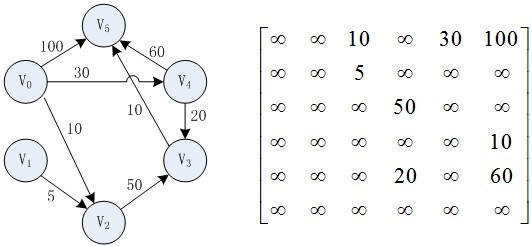
\includegraphics[width=240pt]{dijkstra.png}\\
\figcaption{有向图及其邻接矩阵}\label{fig:dijkstra}
\end{center}

运算过程中$v_0$到其余个顶点的最短路近,\fn{dist[]}向量的变化情况如表\ref{tab:dijkstra}所示(从一列到下一列只需要更新新加入点的邻接点)。

\begin{center}
\tabcaption{Dijkstra算法过程中dist[]向量的变化情况}
\label{tab:dijkstra}
\begin{tabular}{|c|ccccc|}
\hline
\textbf{\textbf{终点}} & \textbf{i=1} & \textbf{i=2} & \textbf{i=3} & \textbf{i=4} & \textbf{i=5}\\
\hline
$v_1$ & $\infty$ & $\infty$ & $\infty$ & $\infty$ & $\infty$\\
\hline
\multirow{2}{*}{$v_2$} & \textbf{10}          & & & & \\
                       & $\mathbf{(v_0,v_2)}$ & & & & \\
\hline
\multirow{2}{*}{$v_3$} & $\infty$ &          60     &     \textbf{50}          & & \\
                       &          & $(v_0,v_2,v_3)$ & $\mathbf{(v_0,v_4,v_5)}$ & & \\
\hline
\multirow{2}{*}{$v_4$} &     30      &      \textbf{30}     & & & \\
                       & $(v_0,v_4)$ & $\mathbf{(v_0,v_4)}$ & & & \\
\hline
\multirow{2}{*}{$v_5$} &     100     &     100     &       90        &         \textbf{60}          & \\
                       & $(v_0,v_5)$ & $(v_0,v_5)$ & $(v_0,v_4,v_5)$ & $\mathbf{(v_0,v_4,v_3,v_5)}$ & \\
\hline
$v_j$ & $v_2$ & $v_4$ & $v_3$ & $v_5$ & \\
\hline
$S$ & $(v_0,v_2)$ & $(v_0,v_2,v_4)$ & $(v_0,v_2,v_3,v_4)$ & $(v_0,v_2,v_3,v_4,v_5)$ & \\
\hline
\end{tabular}
\end{center}

Dijkstra算法的C语言实现如下。

\subsubsection{代码}

\begin{Codex}[label=mgraph_dijkstra.c]
#include <stdio.h>
#include <stdlib.h>  /* for malloc() */
#include <limits.h>  /* for INT_MAX */

/** 顶点数的最大值*/
#define MAX_VERTICES_NUM 100
/** 边的权值,对无权图,用0或1表示是否相邻;对有权图,则为权值. */
typedef int graph_weight_t;
#define GRAPH_INFINITY INT_MAX
/** 顶点信息,例如顶点名字. */
typedef char graph_vertex_t;

/**
 *@struct
 *@brief 邻接矩阵.
 */
typedef struct mgraph_t {
    int vertices_num; /* 顶点数*/
    int edges_num; /* 边数*/
    /* 顶点表,存放顶点的信息,如名字等*/
    graph_vertex_t vertices[MAX_VERTICES_NUM];
    /* 邻接矩阵,存放边的信息,如权重等*/
    graph_weight_t matrix[MAX_VERTICES_NUM][MAX_VERTICES_NUM];
    int directed; /* 图(网)的种类,1表示有向,0表示无向*/
} mgraph_t;

mgraph_t g;

/** path[i]存放的是最短路径上指向vi的弧尾顶点 */
int path[MAX_VERTICES_NUM];
/** dist[i]存放的是v到vi的最短路径长度 */
int dist[MAX_VERTICES_NUM];


/*
  * @brief Dijkstra算法求单源最短路径.
  * @param[in] g 图对象的指针
  * @param[in] v 起点
  * @param[out] dist dist[i]存放的是v到vi的最短路径长度
  * @param[out] path path[i]存放的是最短路径上指向vi的弧尾顶点
  * @return 无
  */
void mgraph_dijkstra(const mgraph_t *g, int v, int dist[], int path[]) {
    int i, j;
    const int n = g->vertices_num;

    // 初始化S集合
    int *S = (int*)malloc( n * sizeof(int));
    for(i = 0; i < n; i++) S[i] = 0;
    S[v] = 1; /* 初始化,顶点u加入S */

    // 初始化dist和path
    for(i = 0; i < n; i++) if (i !=v) {
        dist[i] = g->matrix[v][i];
        if(dist[i] < GRAPH_INFINITY) {
            path[i] = v;
        }  else {
            path[i] = -1; /* 没有顶点指向i */
        }
    }
    dist[v] = 0;
    path[v] = -1;

    for(i = 0; i < n; i++) if (i !=v) {
        /* 选不在S中的最短路径顶点 u */
        int u;
        graph_weight_t min = GRAPH_INFINITY;
        for(j = 0; j < n; j++) {
            if(!S[j] && dist[j] < min) {
                u = j;
                min = dist[j];
            }
        }
        S[u] = 1;
        for(j = 0; j < n; j++) {
            const graph_weight_t w = g->matrix[u][j];
            /* 顶点j未就加入S,且经过u到j可缩短路径*/
            if(!S[j] && w < GRAPH_INFINITY &&
                dist[u] + w < dist[j]) {
                dist[j] = dist[u] + w;
                path[j] = u; /* 修改到j的最短路径*/
            }
        }
    }
    free(S);
}

/*
 * @brief 打印从起点到v的最短路径
 * @param[in] v 终点
 * @param[in] path Dijkstra计算好的path
 * @return 无
 */
static void print_path_r(int v, const int path[]) {
    if (path[v] == -1) {
        printf("%c", g.vertices[v]);
    } else {
        print_path_r(path[v], path);
        printf("->%c", g.vertices[v]);
    }
}

/**
 * @brief 打印 u到其他所有点的最短路径
 * @param[in] path Dijkstra计算好的path
 * @param[in] n path的长度
 * @return 无
 */
void print_path(const int path[], int n) {
    int i;
    for (i = 0; i < n; i++) if (path[i] != -1) {
        print_path_r(i, path);
        printf("\n");
    }
}

/**
 * @brief 读取输入,构建图.
 */
void read_graph() {
    int i, j, k;
    char chx, chy;
    graph_weight_t cost;

    /* 读取节点和边的数目 */
    scanf("%d%d", &(g.vertices_num), &(g.edges_num));
    g.directed = 1;
    for (i = 0; i < g.vertices_num; i++) g.vertices[i] = 'A' + i;

    /* 初始化图,所有节点间距离为无穷大 */
    for (i = 0; i < g.vertices_num; i++) {
        for (j = 0; j < g.vertices_num; j++) {
            g.matrix[i][j] = GRAPH_INFINITY;
        }
    }

    /* 读取边信息 */
    getchar(); // 消耗回车键
    for (k = 0; k < g.edges_num; k++) {
        scanf("%c %c %d", &chx, &chy, &cost);
        getchar();
        i = chx - 'A';
        j = chy - 'A';
        g.matrix[i][j] = cost;
    }
}

/* test

输入数据:

6 8
A C 10
A E 30
A F 100
B C 5
C D 50
D 5 10
E D 20
E F 60

输出:

A->C
A->E->D
A->E
A->E->F
*/
int main() {
    read_graph();

    /* 求 V0 到其他所有顶点的最短路径 */
    mgraph_dijkstra(&g, 0, dist, path);
    print_path(path, g.vertices_num);
    return 0;
}
\end{Codex}

\subsubsection{算法分析}
该算法包含了两个并列的for循环,第一个for循环做辅助数组的初始化工作,计算时间为$O(n)$,第二个for循环是二重嵌套循环,进行最短路径的求解工作,由于对图中几乎每个顶点都要做计算,每个顶点的又要对集合S内的顶点进行检测,对集合$V-S$内中的顶点进行修改,所以运算时间复杂度为$O(n^2)$。算法总的时间复杂度为$O(n^2)$。


\subsection{每点最短路径——Floyd算法}
Floyd算法的基本思想是:假设求从定点$v_i$到$v_j$的最短路径。初始时,若$v_i$与$v_j$之间存在边,则最短路径长度为此边的权值;若不存在边,则最短路径长度为无穷大。以后逐步在路径中加入顶点$k(k=0,1,...,n-1)$作为中间顶点,如果加入中间顶点后,得到的路径比原来的路径长度减少了,则以新路径代替原路径。

首先比较$(v_i,v_j)$和$(v_i,v_0,v_j)$的路径长度,取较短者为从$v_i$到$v_j$的中间顶点的序号不大于0的最短路径。如果$(v_i,v_0,v_j)$较短,则取$(v_i,v_0,v_j)$作为最短路径。假如在路径上再增加一个顶点$v_1$,也就是说,如果$(v_i,...,v_1)$和$(v_1,...,v_j)$分别是当前找到的中间定点的序号不大于0的最短路径,那么$(vi,...,v1,...,vj)$就有可能是从$v_i$到$v_j$的中间顶点的序号不大于1的最短路径,将它和已经得到的从$v_i$到$v_j$的中间顶点的序号不大于0的最短路径相比较,选出较短者作为从$v_i$到$v_j$的中间顶点的序号不大于1的最短路径。再增加一个顶点$v_2$,继续进行试探,依此类推。一般的,若$(v_i,...,v_k)$和$(v_k,...,v_j)$分别是从$v_i$到$v_k$和从$v_k$到$v_j$的中间定点的序号不大于$k-1$的最短路径,则将$(v_i,...,v_k,...,v_j)$和已经得到的从$v_i$到$v_j$的中间顶点的序号不大于$k-1$的最短路径相比,较短者便是从$v_i$到$v_j$的中间顶点的序号不大于$k$的最短路径。这样,在经过$n$次比较后,最后求得的必是从$v_i$到$v_j$的最短路径。

现定义一个$n$阶方阵序列,
$$
D^{(-1)}, D^{(0)} , D^{(1)},..., , D^{(k)},..., , D^{(n-1)}
$$
其中,
\begin{eqnarray}
D^{(-1)}[i][j] &=& \text{g->matrix}[i][j],  \nonumber \\
D^{(k)}[i][j] &=& \min\left\{D^{(k-1)}[i][j], D^{(k-1)}[i][k] + D^{(k-1)}[k][j]\right\},0 \leq k \leq n-1 \nonumber
\end{eqnarray}

上述公式中,$D^{(k)}[i][j]$是从$v_i$到$v_j$的中间顶点的序号不大于$k$的最短路径的长度;$D^{(n-1)}[i][j]$是从$v_i$到$v_j$的最短路径的长度。

例如,对图\ref{fig:floyd}所示的有向图及其邻接矩阵运行Floyd算法,

\begin{center}
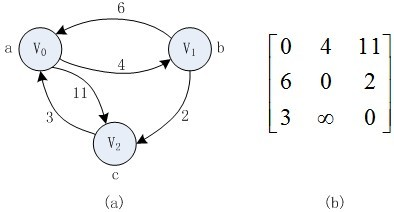
\includegraphics[width=180pt]{floyd.png}\\
\figcaption{有向图及其邻接矩阵}\label{fig:floyd}
\end{center}

运算过程中矩阵D的变化如表\ref{tab:floyd}所示。

\begin{center}
\tabcaption{Floyd算法过程中方阵和最短路径的变化}
\label{tab:floyd}
\begin{tabular}{|c|ccc|ccc|ccc|ccc|}
\hline
\multirow{2}{*}{$\mathbf{D}$} & \multicolumn{3}{|c|}{$\mathbf{D^{(0)}}$} & \multicolumn{3}{|c|}{$\mathbf{D^{(1)}}$} & \multicolumn{3}{|c|}{$\mathbf{D^{(2)}}$} & \multicolumn{3}{|c|}{$\mathbf{D^{(3)}}$} \\
 & 0 & 1 & 2 & 0 & 1 & 2 & 0 & 1 & 2 & 0 & 1 & 2 \\
\hline
0 & 0 & 4 & 11 & 0 & 4 & 11 & 0 & 4 & 6 & 0 & 4 & 6 \\
1 & 6 & 0 & 2 & 6 & 0 & 2 & 6 & 0 & 2 & 5 & 0 & 2 \\
2 & 3 & $\infty$ & 0 & 3 & 7 & 0 & 3 & 7 & 0 & 3 & 7 & 0 \\
\hline
\multirow{2}{*}{$\mathbf{P}$} & \multicolumn{3}{|c|}{$\mathbf{P^{(0)}}$} & \multicolumn{3}{|c|}{$\mathbf{P^{(1)}}$} & \multicolumn{3}{|c|}{$\mathbf{P^{(2)}}$} & \multicolumn{3}{|c|}{$\mathbf{P^{(3)}}$} \\
 & 0 & 1 & 2 & 0 & 1 & 2 & 0 & 1 & 2 & 0 & 1 & 2 \\
\hline
\multirow{2}{*}{0} & & A & A & & AB & A & & AB & AB & & AB & AB \\
                   & & B & C & & & C & & & C & & & C \\
\hline
\multirow{2}{*}{1} & B & & B & B & & B & B & & BC & BC & & BC \\
                   & A & & C & A & & C & A & & & A & & \\
\hline
\multirow{2}{*}{2} & C & & & C & CA & & C & CA & & CA & CA & \\
                   & A & & & A & B & & A & B & & & B & \\
\hline
\end{tabular}
\end{center}

Floyd算法的C语言实现如下。

\subsubsection{代码}

\begin{Codex}[label=mgraph_floyd.c]
#include <stdio.h>
#include <stdlib.h>  /* for malloc() */
#include <limits.h>  /* for INT_MAX */

/** 顶点数的最大值*/
#define MAX_VERTICES_NUM 100
/** 边的权值,对无权图,用0或1表示是否相邻;对有权图,则为权值. */
typedef int graph_weight_t;
#define GRAPH_INFINITY (INT_MAX / 2)   /* 确保加法不溢出 */
/** 顶点信息,例如顶点名字. */
typedef char graph_vertex_t;

/**
 *@struct
 *@brief 邻接矩阵.
 */
typedef struct mgraph_t {
    int vertices_num; /* 顶点数*/
    int edges_num; /* 边数*/
    /* 顶点表,存放顶点的信息,如名字等*/
    graph_vertex_t vertices[MAX_VERTICES_NUM];
    /* 邻接矩阵,存放边的信息,如权重等*/
    graph_weight_t matrix[MAX_VERTICES_NUM][MAX_VERTICES_NUM];
    int directed; /* 图(网)的种类,1表示有向,0表示无向*/
} mgraph_t;


mgraph_t g;
/** dist[i][j]是顶点i和j之间最短路径长度 */
graph_weight_t dist[MAX_VERTICES_NUM][MAX_VERTICES_NUM];
/** path[i][j]是最短路径上i和j之间的顶点 */
int path[MAX_VERTICES_NUM][MAX_VERTICES_NUM];


/*
  * @brief Floyd算法求每点之间最短路径.
  * @param[in] g 图对象的指针
  * @param[out] dist dist[i][j]是顶点i和j之间最短路径长度
  * @param[out] path path[i][j]是最短路径上i和j之间的顶点
  * @return 无
  */
void mgraph_floyd(const mgraph_t *g,
       int dist[][MAX_VERTICES_NUM],
       int path[][MAX_VERTICES_NUM]) {
    int i, j, k;
    const int n = g->vertices_num;

    for(i = 0; i < n; i++) {
        for(j = 0; j < n; j++) {
            if(i != j) {
                dist[i][j] = g->matrix[i][j];
                path[i][j] = i;
            } else {
                dist[i][j] = 0;
                path[i][j] = -1;
            }
        }
    }
    for(k = 0; k < n; k++) {
        for(i = 0; i < n; i++) {
            for(j = 0; j < n; j++) {
                /* i到j的路径上加入顶点k可以缩短路径长度*/
                if(dist[i][k] + dist[k][j] < dist[i][j]) {
                    dist[i][j] = dist[i][k] + dist[k][j];
                    path[i][j] = k;
                }
            }
        }
    }
}

/*
 * @brief 打印从u到v的最短路径
 * @param[in] u 起点
 * @param[in] v 终点
 * @param[in] path Floyd 计算好的path
 * @return 无
 */
static void print_path_r(int u, int v, const int path[][MAX_VERTICES_NUM]) {
    if (path[u][v] == -1) {
        printf("%c", g.vertices[u]);
    } else {
        print_path_r(u, path[u][v], path);
        printf("->%c", g.vertices[v]);
    }
}

/**
 * @brief 打印 u到其他所有点的最短路径
 * @param[in] path Dijkstra计算好的path
 * @param[in] n path的长度
 * @return 无
 */
void print_path(const mgraph_t *g, const int path[][MAX_VERTICES_NUM]) {
    int i, j;
    for (i = 0; i < g->vertices_num; i++) {
        for (j = 0; j < g->vertices_num; j++) {
            if (i != j) {
                print_path_r(i, j, path);
                printf("\n");
            }
        }
        printf("\n");
    }
}


/* test

输入数据:

3 5
A B 4
A C 11
B A 6
B C 2
C A 3

输出:

A->B
A->B->C

B->C->A
B->C

C->A
C->A->B
*/
int main() {
    int i, j, k;
    char chx, chy;
    graph_weight_t cost;

    /* 读取节点和边的数目 */
    scanf("%d%d", &(g.vertices_num), &(g.edges_num ));
    g.directed = 1;
    for (i = 0; i < g.vertices_num; i++) g.vertices[i] = 'A' + i;

    /* 初始化图,所有节点间距离为无穷大 */
    for (i = 0; i < g.vertices_num; i++) {
        for (j = 0; j < g.vertices_num; j++) {
            g.matrix[i][j] = GRAPH_INFINITY;
        }
    }

    /* 读取边信息 */
    getchar(); // 消耗回车键
    for (k = 0; k < g.edges_num ; k++) {
        scanf("%c %c %d", &chx, &chy, &cost);
        getchar();
        i = chx - 'A';
        j = chy - 'A';
        g.matrix[i][j] = cost;
    }

    /* 求两两之间的最短路径 */
    mgraph_floyd(&g, dist, path);
    print_path(&g, path);
    return 0;
}
\end{Codex}

\subsubsection{算法分析}
该算法中有两个并列的for循环,第一个循环是个二重循环,用于初始化方阵$D$;第二个循环是个三重循环,逐步生成$D^{(0)}, D^{(1)} ,...,D^{(n-1)}$。所以算法总的时间复杂度为$O(n^3)$。

Dijkstra算法权值不能为负,Floyd权值可以为负,但环路之和不能为负。


\subsection{例题:HDU 2544 最短路}
\subsubsection{描述}
在每年的校赛里,所有进入决赛的同学都会获得一件很漂亮的t-shirt。但是每当我们的工作人员把上百件的衣服从商店运回到赛场的时候,却是非常累的!所以现在他们想要寻找最短的从商店到赛场的路线,你可以帮助他们吗?

\subsubsection{输入}
输入包括多组数据。每组数据第一行是两个整数$N,M(N \leq 100,M \leq 10000)$,$N$表示成都的大街上有几个路口,标号为1的路口是商店所在地,标号为$N$的路口是赛场所在地,$M$则表示在成都有几条路。$N=M=0$表示输入结束。接下来$M$行,每行包括3个整数$A,B,C(1 \leq A,B \leq N,1 \leq C \leq 1000)$,表示在路口$A$与路口$B$之间有一条路,我们的工作人员需要$C$分钟的时间走过这条路。
输入保证至少存在1条商店到赛场的路线。

\subsubsection{输出}
对于每组输入,输出一行,表示工作人员从商店走到赛场的最短时间

\subsubsection{样例输入}
\begin{Code}
2 1
1 2 3
3 3
1 2 5
2 3 5
3 1 2
0 0
\end{Code}

\subsubsection{样例输出}
\begin{Code}
3
2
\end{Code}

\subsubsection{分析}
单源最短路径,用Dijkstra算法,将第\S\ref{sec:dijkstra}节中的代码稍加修改即可。

注意,街道是双向的,所以给边赋值时要对称赋值。

\subsubsection{代码}
\begin{Codex}[label=hdu_2544.c]
/* http://acm.hdu.edu.cn/showproblem.php?pid=2544 */
#include <stdio.h>
#include <stdlib.h>  /* for malloc() */
#include <limits.h>  /* for INT_MAX */

/** 顶点数的最大值*/
#define MAX_VERTICES_NUM 100
/** 边的权值,对无权图,用0或1表示是否相邻;对有权图,则为权值. */
typedef int graph_weight_t;
#define GRAPH_INFINITY INT_MAX
/** 顶点信息,例如顶点名字. */
typedef char graph_vertex_t;

/**
 *@struct
 *@brief 邻接矩阵.
 */
typedef struct mgraph_t {
    int vertices_num; /* 顶点数*/
    int edges_num; /* 边数*/
    /* 顶点表,存放顶点的信息,如名字等*/
    graph_vertex_t vertices[MAX_VERTICES_NUM];
    /* 邻接矩阵,存放边的信息,如权重等*/
    graph_weight_t matrix[MAX_VERTICES_NUM][MAX_VERTICES_NUM];
    int directed; /* 图(网)的种类,1表示有向,0表示无向*/
} mgraph_t;

mgraph_t g;

/** path[i]存放的是最短路径上指向vi的弧尾顶点 */
int path[MAX_VERTICES_NUM];
/** dist[i]存放的是v到vi的最短路径长度 */
int dist[MAX_VERTICES_NUM];


/*
  * @brief Dijkstra算法求单源最短路径.
  * @param[in] g 图对象的指针
  * @param[in] v 起点
  * @param[out] dist dist[i]存放的是v到vi的最短路径长度
  * @param[out] path path[i]存放的是最短路径上指向vi的弧尾顶点
  * @return 无
  */
void mgraph_dijkstra(const mgraph_t *g, int v, int dist[], int path[]) {
    int i, j;
    const int n = g->vertices_num;

    // 初始化S集合
    int *S = (int*)malloc( n * sizeof(int));
    for(i = 0; i < n; i++) S[i] = 0;
    S[v] = 1; /* 初始化,顶点u加入S */

    // 初始化dist和path
    for(i = 0; i < n; i++) if (i !=v) {
        dist[i] = g->matrix[v][i];
        if(dist[i] < GRAPH_INFINITY) {
            path[i] = v;
        }  else {
            path[i] = -1; /* 没有顶点指向i */
        }
    }
    dist[v] = 0;
    path[v] = -1;

    for(i = 0; i < n; i++) if (i !=v) {
        /* 选不在S中的最短路径顶点 u */
        int u;
        graph_weight_t min = GRAPH_INFINITY;
        for(j = 0; j < n; j++) {
            if(!S[j] && dist[j] < min) {
                u = j;
                min = dist[j];
            }
        }
        S[u] = 1;
        for(j = 0; j < n; j++) {
            const graph_weight_t w = g->matrix[u][j];
            /* 顶点j未就加入S,且经过u到j可缩短路径*/
            if(!S[j] && w < GRAPH_INFINITY &&
                dist[u] + w < dist[j]) {
                dist[j] = dist[u] + w;
                path[j] = u; /* 修改到j的最短路径*/
            }
        }
    }
    free(S);
}

int main() {
    int i, j, k;
    int x, y;
    graph_weight_t cost;

    /* 读取节点和边的数目 */
    while(scanf("%d%d", &(g.vertices_num), &(g.edges_num)) > 0)
        if (g.vertices_num > 0 && g.edges_num > 0){
        g.directed = 1;
        for (i = 0; i < g.vertices_num; i++) g.vertices[i] = '1' + i;

        /* 初始化图,所有节点间距离为无穷大 */
        for (i = 0; i < g.vertices_num; i++) {
            for (j = 0; j < g.vertices_num; j++) {
                g.matrix[i][j] = GRAPH_INFINITY;
            }
        }

        /* 读取边信息 */
        for (k = 0; k < g.edges_num; k++) {
            scanf("%d %d %d", &x, &y, &cost);
            i = x - 1;
            j = y - 1;
            g.matrix[i][j] = cost;
            g.matrix[j][i] = cost;  // 注意,街道是双向的
        }

        /* 求 商店(即路口1) 到其他所有顶点的最短路径 */
        mgraph_dijkstra(&g, 0, dist, path);
        /* 打印商店(即路口1)到赛场(即路口N)的最短路径长度 */
        printf("%d\n", dist[g.vertices_num-1]);
    }
    return 0;
}
\end{Codex}

\subsubsection{相关的题目}
与本题相同的题目:
\begindot
\item HDU 2544 最短路, \myurl{http://acm.hdu.edu.cn/showproblem.php?pid=2544}
\myenddot

与本题相似的题目:
\begindot
\item POJ 2253 Frogger, \myurl{http://poj.org/problem?id=2253}
\item POJ 3268 Silver Cow Party, \myurl{http://poj.org/problem?id=3268}
\item POJ 1797 Heavy Transportation, \myurl{http://poj.org/problem?id=1797}
\item POJ 1847 Tram, \myurl{http://poj.org/problem?id=1847}
\myenddot


\subsection{例题:POJ 1125 Stockbroker Grapevine}
\subsubsection{描述}
Stockbrokers are known to overreact to rumours. You have been contracted to develop a method of spreading disinformation amongst the stockbrokers to give your employer the tactical edge in the stock market. For maximum effect, you have to spread the rumours in the fastest possible way. 

Unfortunately for you, stockbrokers only trust information coming from their "Trusted sources" This means you have to take into account the structure of their contacts when starting a rumour. It takes a certain amount of time for a specific stockbroker to pass the rumour on to each of his colleagues. Your task will be to write a program that tells you which stockbroker to choose as your starting point for the rumour, as well as the time it will take for the rumour to spread throughout the stockbroker community. This duration is measured as the time needed for the last person to receive the information.

\subsubsection{输入}
Your program will input data for different sets of stockbrokers. Each set starts with a line with the number of stockbrokers. Following this is a line for each stockbroker which contains the number of people who they have contact with, who these people are, and the time taken for them to pass the message to each person. The format of each stockbroker line is as follows: The line starts with the number of contacts ($n$), followed by n pairs of integers, one pair for each contact. Each pair lists first a number referring to the contact (e.g. a '1' means person number one in the set), followed by the time in minutes taken to pass a message to that person. There are no special punctuation symbols or spacing rules. 

Each person is numbered 1 through to the number of stockbrokers. The time taken to pass the message on will be between 1 and 10 minutes (inclusive), and the number of contacts will range between 0 and one less than the number of stockbrokers. The number of stockbrokers will range from 1 to 100. The input is terminated by a set of stockbrokers containing 0 (zero) people. 

\subsubsection{输出}
For each set of data, your program must output a single line containing the person who results in the fastest message transmission, and how long before the last person will receive any given message after you give it to this person, measured in integer minutes. 

It is possible that your program will receive a network of connections that excludes some persons, i.e. some people may be unreachable. If your program detects such a broken network, simply output the message "disjoint". Note that the time taken to pass the message from person A to person B is not necessarily the same as the time taken to pass it from B to A, if such transmission is possible at all.

\subsubsection{样例输入}
\begin{Code}
3
2 2 4 3 5
2 1 2 3 6
2 1 2 2 2
5
3 4 4 2 8 5 3
1 5 8
4 1 6 4 10 2 7 5 2
0
2 2 5 1 5
7        
2 2 6 7 1
0  
3 1 5 2 8 4 7
0
2 2 9 4 10
2 3 8 4 7
2 5 8 6 3
7        
2 2 6 7 8
0  
3 1 5 2 8 4 7
0
2 2 9 4 10
2 3 8 4 7
2 5 8 6 3
0
\end{Code}

\subsubsection{样例输出}
\begin{Code}
3 2  
3 10
1 12
7 17
\end{Code}

\subsubsection{分析}

\subsubsection{代码}
\begin{Codex}[label=poj_1125.c]
/* http://poj.org/problem?id=1125 */
#include <stdio.h>
#include <stdlib.h>  /* for malloc() */
#include <limits.h>  /* for INT_MAX */

/** 顶点数的最大值*/
#define MAX_VERTICES_NUM 100
/** 边的权值,对无权图,用0或1表示是否相邻;对有权图,则为权值. */
typedef int graph_weight_t;
#define GRAPH_INFINITY (INT_MAX / 2)   /* 确保加法不溢出 */
/** 顶点信息,例如顶点名字. */
typedef char graph_vertex_t;

/**
 *@struct
 *@brief 邻接矩阵.
 */
typedef struct mgraph_t {
    int vertices_num; /* 顶点数*/
    int edges_num; /* 边数*/
    /* 顶点表,存放顶点的信息,如名字等*/
    graph_vertex_t vertices[MAX_VERTICES_NUM];
    /* 邻接矩阵,存放边的信息,如权重等*/
    graph_weight_t matrix[MAX_VERTICES_NUM][MAX_VERTICES_NUM];
    int directed; /* 图(网)的种类,1表示有向,0表示无向*/
} mgraph_t;


mgraph_t g;
/** dist[i][j]是顶点i和j之间最短路径长度 */
graph_weight_t dist[MAX_VERTICES_NUM][MAX_VERTICES_NUM];
/** path[i][j]是最短路径上i和j之间的顶点 */
int path[MAX_VERTICES_NUM][MAX_VERTICES_NUM];
/** 存放每个点的最短路径的最长者 */
graph_weight_t max_len[MAX_VERTICES_NUM];

/**
  * @brief Floyd算法求每点之间最短路径.
  * @param[in] g 图对象的指针
  * @param[out] dist dist[i][j]是顶点i和j之间最短路径长度
  * @param[out] path path[i][j]是最短路径上i和j之间的顶点
  * @return 无
  */
void mgraph_floyd(const mgraph_t *g,
       int dist[][MAX_VERTICES_NUM],
       int path[][MAX_VERTICES_NUM]) {
    int i, j, k;
    const int n = g->vertices_num;

    for(i = 0; i < n; i++) {
        for(j = 0; j < n; j++) {
            if(i != j) {
                dist[i][j] = g->matrix[i][j];
                path[i][j] = i;
            } else {
                dist[i][j] = 0;
                path[i][j] = -1;
            }
        }
    }
    for(k = 0; k < n; k++) {
        for(i = 0; i < n; i++) {
            for(j = 0; j < n; j++) {
                /* i到j的路径上加入顶点k可以缩短路径长度*/
                if(dist[i][k] + dist[k][j] < dist[i][j]) {
                    dist[i][j] = dist[i][k] + dist[k][j];
                    path[i][j] = k;
                }
            }
        }
    }
}

static int max_element(const graph_weight_t w[], int begin, int end) {
    int i;
    int max_value = INT_MIN;
    int max_pos = -1;
    for (i = begin; i < end; i++) {
        if (max_value < w[i]) {
            max_value = w[i];
            max_pos = i;
        }
    }
    return max_pos;
}

static int min_element(const graph_weight_t w[], int begin, int end) {
    int i;
    int min_value = INT_MAX;
    int min_pos = -1;
    for (i = begin; i < end; i++) {
        if (min_value > w[i]) {
            min_value = w[i];
            min_pos = i;
        }
    }
    return min_pos;
}

int main() {
    int i, j;
    int min_pos;

    /* 读取顶点数 */
    while (scanf("%d", &(g.vertices_num)) > 0 && g.vertices_num > 0) {
        g.edges_num = 0;
        g.directed = 1;
        for (i = 0; i < g.vertices_num; i++) g.vertices[i] = '1' + i;

        /* 初始化图,所有节点间距离为无穷大 */
        for (i = 0; i < g.vertices_num; i++) {
            for (j = 0; j < g.vertices_num; j++) {
                g.matrix[i][j] = GRAPH_INFINITY;
            }
        }

        /* 读取边信息 */
        for (i = 0; i < g.vertices_num; i++) {
            int m;
            graph_weight_t cost;
            scanf("%d", &m);
            g.edges_num += m;
            while (m--) {
                scanf("%d %d", &j, &cost);
                --j;
                g.matrix[i][j] = cost;
            }
        }

        /* 求两两之间的最短路径 */
        mgraph_floyd(&g, dist, path);

        /* 找最短路径的最长着 */
        for (i = 0; i < g.vertices_num; i++) {
            max_len[i] = dist[i][max_element(dist[i], 0, g.vertices_num)];
        }
        /* 找 max_len 的最小者 */
        min_pos = min_element(max_len, 0, g.vertices_num);

        if (max_len[min_pos] == GRAPH_INFINITY) {
            printf("disjoint\n");
        } else {
            printf("%d %d\n", min_pos+1, max_len[min_pos]);
        }
    }
    return 0;
}
\end{Codex}

\subsubsection{相关的题目}
与本题相同的题目:
\begindot
\item POJ 1125 Stockbroker Grapevine, \myurl{http://poj.org/problem?id=1125}
\myenddot

与本题相似的题目:
\begindot
\item POJ 3615 Cow Hurdles, \myurl{http://poj.org/problem?id=3615}
\item POJ 3660 Cow Contest, \myurl{http://poj.org/problem?id=3660}
\item POJ 2502 Subway, \myurl{http://poj.org/problem?id=2502}
\item HDU 3631 Shortest Path, \myurl{http://acm.hdu.edu.cn/showproblem.php?pid=3631}
\myenddot


\section{拓扑排序} %%%%%%%%%%%%%%%%%%%%%%%%%%%%%%
由某个集合上的一个偏序得到该集合上的一个全序,这个操作称为\textbf{拓扑排序}。

拓扑序列的特点是:若有向边$<V_i, V_j>$是途中的弧,则在序列中顶点$V_i$必须排在顶点$V_j$之前。

如果用有向图表示一个工程,顶点表示活动,用有向边$<v_i,v_j>$表示活动必须先于活动进行。这种有向图叫做顶点表示活动的网络(Activity On Vertext Network),简称\textbf{AOV网络}。

检测AOV网络是否存在环的方法是对AOV网络构造其顶点的拓扑有序序列。拓扑排序的基本步骤是:
\begin{enumerate}
\item 在有向图中选一个没有前驱的顶点且输出之;
\item 从图中删除该顶点和所有以它为尾的弧线。
\end{enumerate}
重复以上两步,直至全部顶点输出,或当前图中不存在无前驱的顶点为止(这种情况说明图中存在环)。

拓扑排序的C语言实现如下。

\subsubsection{代码}

\begin{Codex}[label=mgraph_topo_sort.c]
#include <stdio.h>
#include <stdlib.h>  /* for malloc() */
#include <limits.h>  /* for INT_MAX */

/** 顶点数的最大值*/
#define MAX_VERTICES_NUM 100
/** 边的权值,对无权图,用0或1表示是否相邻;对有权图,则为权值. */
typedef int graph_weight_t;
#define GRAPH_INFINITY INT_MAX
/** 顶点信息,例如顶点名字. */
typedef char graph_vertex_t;

/**
 *@struct
 *@brief 邻接矩阵.
 */
typedef struct mgraph_t {
    int vertices_num; /* 顶点数*/
    int edges_num; /* 边数*/
    /* 顶点表,存放顶点的信息,如名字等*/
    graph_vertex_t vertices[MAX_VERTICES_NUM];
    /* 邻接矩阵,存放边的信息,如权重等*/
    graph_weight_t matrix[MAX_VERTICES_NUM][MAX_VERTICES_NUM];
    int directed; /* 图(网)的种类,1表示有向,0表示无向*/
} mgraph_t;

mgraph_t g;
/** 拓扑排序的结果. */
int topological[MAX_VERTICES_NUM];

// 等价于复制粘贴,这里为了节约篇幅,使用include,在OJ上提交时请用复制粘贴
#include "stack.c"

/*
  * @brief 拓扑排序.
  * @param[in] g 图对象的指针
  * @param[out] topological 保存拓扑排序的结果
  * @return 无环返回 1,有环返回 0
  */
int mgraph_topo_sort(const mgraph_t *g, int topological[]) {
    int i, j, u;
    int count = 0; /* 拓扑序列的元素个数*/
    const int n = g->vertices_num;
    /* in_degree[i]是顶点i的入度 */
    int *in_degree = (int*)malloc(n * sizeof(int));
    stack_t s;

    memset(in_degree, 0, n * sizeof(int));
    for (i = 0; i < n; i++) {
        for (j = 0; j < n; j++) {
            if (g->matrix[i][j] < GRAPH_INFINITY)
                in_degree[j]++;
        }
    }

    stack_init(&s, n * sizeof(int));
    for(i = 0; i < n; i ++) {
        if(in_degree[i] == 0)
            stack_push(&s, i);
    }

    while(!stack_empty(&s)) {
        u = stack_top(&s); stack_pop(&s);
        topological[count++] = u;
        for (i = 0; i < n; i++) if (g->matrix[u][i] < GRAPH_INFINITY) {
            if(--in_degree[i] == 0) stack_push(&s, i);
        }
    }

    free(in_degree);
    if(count != n) { /* 有环*/
        return 0;
    } else { /* 无环*/
        return 1;
    }
}


/* test

输入数据:

6 8
A C 10
A E 30
A F 100
B C 5
C D 50
D 5 10
E D 20
E F 60

输出:

B A E F C D
*/
int main() {
    int i, j, k;
    char chx, chy;
    graph_weight_t cost;

    /* 读取节点和边的数目 */
    scanf("%d%d", &(g.vertices_num), &(g.edges_num));
    getchar(); // 消耗回车键
    g.directed = 1;
    for (i = 0; i < g.vertices_num; i++) g.vertices[i] = 'A' + i;

    /* 初始化图,所有节点间距离为无穷大 */
    for (i = 0; i < g.vertices_num; i++) {
        for (j = 0; j < g.vertices_num; j++) {
            g.matrix[i][j] = GRAPH_INFINITY;
        }
    }

    /* 读取边信息 */
    for (k = 0; k < g.edges_num; k++) {
        scanf("%c %c %d", &chx, &chy, &cost);
        getchar();
        i = chx - 'A';
        j = chy - 'A';
        g.matrix[i][j] = cost;
    }

    /* 拓扑排序 */
    mgraph_topo_sort(&g, topological);
    for (i = 0; i < g.vertices_num; i++) {
        printf("%c ", g.vertices[topological[i]]);
    }
    return 0;
}
\end{Codex}

\subsubsection{算法分析}
对有$n$个顶点和$e$条边的AOV网络而言,求各顶点的入度所需时间为$O(e)$,建立零入度顶点栈所需时间为$O(n)$;在拓扑排序过程中,若有向图无环,每个顶进一次栈出一次栈,顶点入度减1的操作共执行了$e$次。所以总的时间复杂度为$O(n+e)$。

当有向图中无环时,也可以利用深度优先搜索进行拓扑排序。因为图中无环,深度优先遍历不会死循环。进行深度优先遍历时,最先退出DFS函数的顶点即为出度为零的顶点,是拓扑有序序列的最后一个顶点。由此,按退出DFS函数的先后次序记录下来的顶点序列即为逆向的拓扑有序序列。


\subsection{例题:POJ 1094 Sorting It All Out}
\subsubsection{描述}
An ascending sorted sequence of distinct values is one in which some form of a less-than operator is used to order the elements from smallest to largest. For example, the sorted sequence $A, B, C, D$ implies that $A < B, B < C$ and $C < D$. in this problem, we will give you a set of relations of the form $A < B$ and ask you to determine whether a sorted order has been specified or not.

\subsubsection{输入}
Input consists of multiple problem instances. Each instance starts with a line containing two positive integers $n$ and $m$. the first value indicated the number of objects to sort, where $2 \leq n \leq 26$. The objects to be sorted will be the first $n$ characters of the uppercase alphabet. The second value $m$ indicates the number of relations of the form $A < B$ which will be given in this problem instance. Next will be $m$ lines, each containing one such relation consisting of three characters: an uppercase letter, the character "<" and a second uppercase letter. No letter will be outside the range of the first $n$ letters of the alphabet. Values of $n = m = 0$ indicate end of input.

\subsubsection{输出}
For each problem instance, output consists of one line. This line should be one of the following three: 

Sorted sequence determined after $xxx$ relations: $yyy...y$.

Sorted sequence cannot be determined. 

Inconsistency found after $xxx$ relations.

where $xxx$ is the number of relations processed at the time either a sorted sequence is determined or an inconsistency is found, whichever comes first, and $yyy...y$ is the sorted, ascending sequence.

\subsubsection{样例输入}
\begin{Code}
4 6
A<B
A<C
B<C
C<D
B<D
A<B
3 2
A<B
B<A
26 1
A<Z
6 6
A<F
B<D
C<E
F<D
D<E
E<F
0 0
\end{Code}

\subsubsection{样例输出}
\begin{Code}
Sorted sequence determined after 4 relations: ABCD.
Inconsistency found after 2 relations.
Sorted sequence cannot be determined.
Inconsistency found after 6 relations.
\end{Code}

\subsubsection{分析}
根据题目的要求,我们要每输入一次就要进行一次拓扑排序\fn{topological_sort()},这样才能做到不成功(即发现有环)时,能知道是哪步不成功,并且给出输出。

还有要注意的就是如果我们可以提前判断结果了,但后面还有输入没完成,那么我们必须继续完成输入,不然剩下的输入会影响下一次case的输入。

\subsubsection{代码}
\begin{Codex}[label=poj_1094.c]
#include <stdio.h>
#include <stdlib.h>  /* for malloc() */
#include <limits.h>  /* for INT_MAX */

/** 顶点数的最大值*/
#define MAX_VERTICES_NUM 26
/** 边的权值,对无权图,用0或1表示是否相邻;对有权图,则为权值. */
typedef int graph_weight_t;
#define GRAPH_INFINITY INT_MAX
/** 顶点信息,例如顶点名字. */
typedef char graph_vertex_t;

/**
 *@struct
 *@brief 邻接矩阵.
 */
typedef struct mgraph_t {
    int vertices_num; /* 顶点数*/
    int edges_num; /* 边数*/
    /* 顶点表,存放顶点的信息,如名字等*/
    graph_vertex_t vertices[MAX_VERTICES_NUM];
    /* 邻接矩阵,存放边的信息,如权重等*/
    graph_weight_t matrix[MAX_VERTICES_NUM][MAX_VERTICES_NUM];
    int directed; /* 图(网)的种类,1表示有向,0表示无向*/
} mgraph_t;

mgraph_t g;
/** 拓扑排序的结果. */
int topological[MAX_VERTICES_NUM];

// 等价于复制粘贴,这里为了节约篇幅,使用include,在OJ上提交时请用复制粘贴
#include "stack.c"

/**
  * @brief 拓扑排序.
  * @param[in] g 图对象的指针
  * @param[out] topological 保存拓扑排序的结果
  * @return 无环返回 1,有环返回 0
  */
int mgraph_topological_sort(const mgraph_t *g, int topological[]) {
    int i, j, u;
    int count = 0; /* 拓扑序列的元素个数*/
    int insufficient = 0;  /* 条件不足 */
    const int n = g->vertices_num;
    /* in_degree[i]是顶点i的入度 */
    int *in_degree = (int*)malloc(n * sizeof(int));
    stack_t s;

    memset(in_degree, 0, n * sizeof(int));
    for (i = 0; i < n; i++) {
        for (j = 0; j < n; j++) {
            if (g->matrix[i][j] < GRAPH_INFINITY)
                in_degree[j]++;
        }
    }

    stack_init(&s, n * sizeof(int));
    for(i = 0; i < n; i ++) {
        if(in_degree[i] == 0) {
            stack_push(&s, i);
        }
    }

    while(!stack_empty(&s)) {
        // 栈内应该始终只有一个元素
        if (stack_size(&s) > 1) insufficient = 1;
        // 删除顶点u
        u = stack_top(&s); stack_pop(&s);
        topological[count++] = u;
        --in_degree[u];  // 变成 -1,表示已经输出
        // 更新入度
        for (i = 0; i < n; i++) if (g->matrix[u][i] < GRAPH_INFINITY) {
            --in_degree[i];
        }
        // 选择入度为0的顶点
        for (i = 0; i < n; i++) if (g->matrix[u][i] < GRAPH_INFINITY) {
            if (in_degree[i] == 0) stack_push(&s, i);
        }
    }

    free(in_degree);
    if(count < n) { /* 有环*/
        return 0;
    } else { /* 无环*/
        if (insufficient) {  /* 有孤立点,说明条件不足 */
            return -1;
        } else {
            return 1;
        }
    }
}


int main() {
    int i, j, k, m;  // m不一定是边的数目,因为输入边可能有重复

    /* 读取节点和边的数目 */
    while (scanf("%d %d", &(g.vertices_num), &m)
            && g.vertices_num > 0 && m > 0) {
        char s[4];
        int ok;  // 是否有环,0 表示有环
        int finished = 0;  // 排序完成,结束,发现有环,可以提前结束

        g.directed = 1;
        for (i = 0; i < g.vertices_num; i++) g.vertices[i] = 'A' + i;

        /* 初始化图,所有节点间距离为无穷大 */
        for (i = 0; i < g.vertices_num; i++) {
            for (j = 0; j < g.vertices_num; j++) {
                g.matrix[i][j] = GRAPH_INFINITY;
            }
        }

        /* 读取边信息 */
        for (k = 0; k < m; k++) {
            scanf("%s", s);
            i = s[0] - 'A';
            j = s[2] - 'A';
            g.matrix[i][j] = 1;

            if (finished) continue;    // 完成,则 continue,消耗输入

            /* 拓扑排序 */
            ok = mgraph_topological_sort(&g, topological);

            if (ok == 0) {  // 有环存在
                printf("Inconsistency found after %d relations.\n", k + 1);
                finished = 1;  // 提前结束,记住要继续消耗输入
            }
            if (ok == 1 && k) {
                printf("Sorted sequence determined after %d relations: ", k+1);
                for (i = 0; i < g.vertices_num; i++) {
                    printf("%c", g.vertices[topological[i]]);
                }
                printf(".\n");
                finished = 1;
            }
            // ok==-1, continue
        }
        if (finished == 0) {
            printf("Sorted sequence cannot be determined.\n");
        }
    }
    return 0;
}
\end{Codex}

\subsubsection{相关的题目}
与本题相同的题目:
\begindot
\item POJ 1094 Sorting It All Out, \myurl{http://poj.org/problem?id=1094}
\myenddot

与本题相似的题目:
\begindot
\item POJ 3267 The Cow Lexicon, \myurl{http://poj.org/problem?id=3267}
\item POJ 3687 Labeling Balls, \myurl{http://poj.org/problem?id=3687}
\myenddot


\section{关键路径} %%%%%%%%%%%%%%%%%%%%%%%%%%%%%%
用有向边上的权值表示活动的持续时间,用顶点表示时间,这样的有向图叫做边表示的活动网络(Activity On Edge Network),简称\textbf{AOE网络}。

路径最长的路径叫做\textbf{关键路径}(Critical Path)。假设开始点为$v_1$,从$v_1$到$v_i$的最长路径长度叫做事件$v_i$的最早发生时间。这个事件决定了所有以$v_i$为尾的弧所表示的活动的最早开始时间。我们用$e(i)$表示活动$a_i$的最早开始时间。还可以定义一个活动的最迟开始时间$l(i)$,这是在不推迟整个工程完成的前提下,活动$a_i$最迟必须开始进行的时间。两者之差$l(i)-e(i)$意味着完成活动$a_i$的时间余量。我们把$l(i)=e(i)$的活动叫做关键活动。

设活动$a_i$由弧$<j, k>$表示,为了求得活动的$e(i)$和$l(i)$,首先应求得事件的最早发生时间$ve(j)$和最迟发生时间$vl(j)$,其持续时间记为$dut(<j, k>)$,则有如下关系
\begin{eqnarray}
e(i) &=& ve(j) \nonumber \\
l(i) &=& vl(k)-dut(<j, k>) \nonumber
\end{eqnarray}

求$ve(j)$和$vl(k)$需分两步进行:
\begin{enumerate}
\item 从$ve(0)=0$开始向前递推
$$
ve(j)=\max\left\{ve(i)+dut(<i, j>)\right\}, <i, j> \in T
$$
其中$T$是所有以顶点$j$为弧头的边的集合。
\item 从$vl(n-1)=ve(n-1)$起向后递推
$$
vl(j)=\min\left\{vl(k)-dut(<j, k>)\right\}, <j, k> \in S
$$
其中$S$是所有以顶点$j$为弧尾的边的集合。
\end{enumerate}

例如,对图\ref{fig:criticalpath}(a)所示AOE网络的计算过程如表\ref{tab:criticalpath}所示,可见$a_2$、$a_5$和$a_7$为关键活动,组成一条从起点到终点的关键路径,如图\ref{fig:criticalpath}(b)所示。

\begin{center}
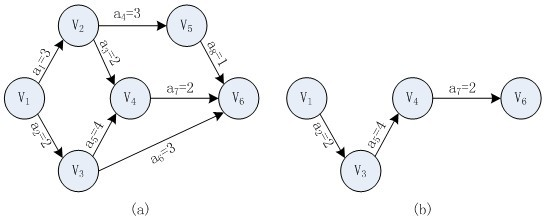
\includegraphics[width=240pt]{criticalpath.png}\\
\figcaption{有向图及其邻接矩阵}\label{fig:criticalpath}
\end{center}

\begin{center}
\tabcaption{图\ref{fig:criticalpath}(a)所示AOE网络的关键路径的计算过程}
\label{tab:criticalpath}
\begin{tabular}{|ccccc|cccc|}
\hline
\textbf{顶点} & \textbf{ve} & & \textbf{vl} & & \textbf{活动} & \textbf{e} & \textbf{l} & \textbf{l-e} \\
\hline
$v_1$ & 0 & \multirow{8}{*}{$\downarrow$} & 0 & \multirow{8}{*}{$\uparrow$} & $a_1$ & 0 & 1 & 1 \\
$v_2$ & 3 &                               & 4 &                             & $a_2$ & 0 & 0 & 0 \\
$v_3$ & 2 &                               & 2 &                             & $a_3$ & 3 & 4 & 1 \\
$v_4$ & 6 &                               & 6 &                             & $a_4$ & 3 & 4 & 1 \\
$v_5$ & 6 &                               & 7 &                             & $a_5$ & 2 & 2 & 0 \\
$v_6$ & 8 &                               & 8 &                             & $a_6$ & 2 & 5 & 3 \\
      &   &                               &   &                             & $a_7$ & 6 & 6 & 0 \\
      &   &                               &   &                             & $a_8$ & 6 & 7 & 1 \\
\hline
\end{tabular}
\end{center}


邻接矩阵上的关键路径的C语言实现如下。

\subsubsection{代码}

\begin{Codex}[label=mgraph_critical_path.c]
#include <stdio.h>
#include <stdlib.h>  /* for malloc() */
#include <limits.h>  /* for INT_MAX */

/** 顶点数的最大值*/
#define MAX_VERTICES_NUM 100
/** 边的权值,对无权图,用0或1表示是否相邻;对有权图,则为权值. */
typedef int graph_weight_t;
#define GRAPH_INFINITY INT_MAX
/** 顶点信息,例如顶点名字. */
typedef char graph_vertex_t;

/**
 *@struct
 *@brief 邻接矩阵.
 */
typedef struct mgraph_t {
    int vertices_num; /* 顶点数*/
    int edges_num; /* 边数*/
    /* 顶点表,存放顶点的信息,如名字等*/
    graph_vertex_t vertices[MAX_VERTICES_NUM];
    /* 邻接矩阵,存放边的信息,如权重等*/
    graph_weight_t matrix[MAX_VERTICES_NUM][MAX_VERTICES_NUM];
    int directed; /* 图(网)的种类,1表示有向,0表示无向*/
} mgraph_t;

mgraph_t g;
/** 拓扑排序的结果. */
int topological[MAX_VERTICES_NUM];
/** 关键路径,其余顶点为-1. */
int path[MAX_VERTICES_NUM];


/* 等价于复制粘贴,这里为了节约篇幅,使用include,在OJ上提交时请用复制粘贴 */
#include "stack.c"


/*
  * @brief 按照拓扑排序的顺序,计算所有顶点的最早发生时间 ve.
  * @param[in] g 图对象的指针
  * @param[out] topological 保存拓扑排序的结果
  * @param[out] ve 所有事件的最早发生时间
  * @return 无环返回 1,有环返回 0
  */
static int mgraph_toposort_ve(const mgraph_t *g, int topological[],
        graph_weight_t ve[]) {
    int i, j, u;
    int count = 0; /* 拓扑序列的元素个数*/
    const int n = g->vertices_num;
    /* in_degree[i]是顶点i的入度 */
    int *in_degree = (int*)malloc(n * sizeof(int));
    stack_t s;

    memset(in_degree, 0, n * sizeof(int));
    for (i = 0; i < n; i++) {
        for (j = 0; j < n; j++) {
            if (g->matrix[i][j] < GRAPH_INFINITY)
                in_degree[j]++;
        }
    }

    stack_init(&s, n * sizeof(int));
    for(i = 0; i < n; i ++) {
        if(in_degree[i] == 0) {
            stack_push(&s, i);
        }
    }

    memset(ve, 0, n * sizeof(graph_weight_t));

    while(!stack_empty(&s)) {
        // 删除顶点u
        u = stack_top(&s); stack_pop(&s);
        topological[count++] = u;
        --in_degree[u];  // 变成 -1,表示已经输出
        // 更新入度
        for (i = 0; i < n; i++) if (g->matrix[u][i] < GRAPH_INFINITY) {
            --in_degree[i];
        }
        // 更新邻接点的 ve
        for (i = 0; i < n; i++) if (g->matrix[u][i] < GRAPH_INFINITY) {
            if (ve[i] < ve[u] + g->matrix[u][i])
                ve[i] = ve[u] + g->matrix[u][i];
        }
        // 选择入度为0的顶点
        for (i = 0; i < n; i++) if (g->matrix[u][i] < GRAPH_INFINITY) {
            if (in_degree[i] == 0) stack_push(&s, i);
        }
    }

    free(in_degree);
    if(count < n) { /* 有环*/
        return 0;
    } else { /* 无环*/
        return 1;
    }
}

/**
  * @brief 求关键路径,第一个顶点为起点,最后一个顶点为终点.
  * @param[in] g 图对象的指针
  * @param[out] ve 所有事件的最早发生时间
  * @param[inout] path 关键路径
  * @return 无环返回关键路径的顶点个数,有环返回 0
  */
int mgraph_critical_path(const mgraph_t *g, int path[MAX_VERTICES_NUM]) {
    int i, j;
    int count = 0;    // 关键路径的顶点个数
    graph_weight_t *ve = (graph_weight_t*) malloc(
            g->vertices_num * sizeof(graph_weight_t));
    graph_weight_t *vl = (graph_weight_t*) malloc(
            g->vertices_num * sizeof(graph_weight_t));

    if (!mgraph_toposort_ve(g, topological, ve)) return 0;  // 有环

    for (i = 0; i < MAX_VERTICES_NUM; i++) path[i] = -1;
    // 初始化 vl 为最大
    for (i = 0; i < g->vertices_num; i++) vl[i] = ve[g->vertices_num-1];

    // 逆序计算vl
    for (i = g->vertices_num-1; i >=0; i--) {
        int k = topological[i];
        for (j = 0; j < g->vertices_num; j++) {
            if (g->matrix[j][k] < GRAPH_INFINITY) {
                if (vl[j] > vl[k] - g->matrix[j][k])
                    vl[j] = vl[k] - g->matrix[j][k];
            }
        }
    }
    for (i = 0; i < g->vertices_num; i++) {
        for (j = 0; j < g->vertices_num; j++) {
            int e = ve[i];
            int l = vl[j] - g->matrix[i][j];
            if (e == l) {
                if (i == 0) {
                    path[count++] = i;
                    path[count++] = j;
                } else {
                    path[count++] = j;
                }
            }
        }
    }

    free(ve);
    free(vl);
    return count;
}


/* test

输入数据:
6 8
A B 3
A C 2
C D 4
B D 2
C F 3
B E 3
E F 1
D F 2

输出: A C D F

*/
int main() {
    int i, j, k;
    char chx, chy;
    graph_weight_t cost;
    int count;

    /* 读取节点和边的数目 */
    scanf("%d%d", &(g.vertices_num), &(g.edges_num));
    g.directed = 1;
    for (i = 0; i < g.vertices_num; i++) g.vertices[i] = 'A' + i;

    /* 初始化图,所有节点间距离为无穷大 */
    for (i = 0; i < g.vertices_num; i++) {
        for (j = 0; j < g.vertices_num; j++) {
            g.matrix[i][j] = GRAPH_INFINITY;
        }
    }

    /* 读取边信息 */
    getchar(); // 消耗回车键
    for (k = 0; k < g.edges_num; k++) {
        scanf("%c %c %d", &chx, &chy, &cost);
        getchar();
        i = chx - 'A';
        j = chy - 'A';
        g.matrix[i][j] = cost;
    }

    /* 拓扑排序 */
    count = mgraph_critical_path(&g, path);
    for (i = 0; i < count; i++) {
        printf("%c ", g.vertices[path[i]]);
    }
    return 0;
}
\end{Codex}

\subsubsection{算法分析}
一次正向,复杂度为$O(n^2)$,一次逆向,复杂度为$O(n^2)$,因此,该算法的复杂度为$O(n^2)$。
